% !TEX TS-program = xelatex
% !TEX encoding = UTF-8 Unicode
\documentclass[12pt,a4paper]{article}

\IfFileExists{src/libs/body.tex}{% --- body.tex ---
\usepackage{pdfpages}
\usepackage{fontspec}
% Prefer Times New Roman when available; fall back in container environments.
\IfFontExistsTF{Times New Roman}{
  \setmainfont{Times New Roman}
}{
  \setmainfont{Liberation Serif}
}
\usepackage[vietnamese]{babel}

% Page layout and spacing
\usepackage[left=3cm,right=2cm,top=2cm,bottom=2cm]{geometry}
\usepackage{titlesec}
\usepackage{setspace}

% Silence noisy warnings
\usepackage{silence}
\WarningFilter{transparent}{Loading aborted}
\WarningFilter{hyperref}{The anchor of a bookmark and its parent's}

% Core packages
\usepackage{float}
\usepackage{svg}
\usepackage{graphicx}
\graphicspath{{assets/}{../assets/}{../../assets/}}
\svgpath{{assets/}{../assets/}{../../assets/}}
\usepackage{enumitem}
\usepackage{array}
\usepackage{tabularx}
\usepackage{multirow}
\usepackage[table]{xcolor}
\usepackage{ulem}
\usepackage{xurl}

% ====== THÊM 2 GÓI NÀY ĐỂ FIX LỖI ADJUSTBOX VÀ FOREST ======
\usepackage{adjustbox}
\usepackage[edges]{forest}
% ============================================================

% TikZ
\usepackage{tikz}

% ====== BỔ SUNG FIT, BACKGROUNDS, TREES VÀO DANH SÁCH ======
\usetikzlibrary{calc, arrows.meta, shapes.geometric, positioning, fit, backgrounds, trees}

% Table tuning
\renewcommand{\tabularxcolumn}[1]{m{#1}}
\hbadness=10000
\hfuzz=10000pt

% Shared commands
\newcommand{\subsecheading}[1]{%
    \par\vspace{2pt}%
    \hspace{1.5em}\textbf{#1}%
    \par\vspace{2pt}%
}
\newcommand{\introtext}[1]{%
    \par\hspace{3.0em}#1\par%
}
\newcommand{\StandaloneDocumentSetup}[2]{%
  \pagenumbering{arabic}%
  \ApplyStandardFooter{#1}{#2}%
}
\newcommand{\StandaloneSectionSetup}[2]{%
  \ApplyStandardFooter{#1}{#2}%
}

% Math
\usepackage{amsmath}

% Hyperref
\usepackage{hyperref}
\hypersetup{
    colorlinks=true,
    linkcolor=black,
    filecolor=magenta,
    urlcolor=blue,
}}{% --- body.tex ---
\usepackage{pdfpages}
\usepackage{fontspec}
% Prefer Times New Roman when available; fall back in container environments.
\IfFontExistsTF{Times New Roman}{
  \setmainfont{Times New Roman}
}{
  \setmainfont{Liberation Serif}
}
\usepackage[vietnamese]{babel}

% Page layout and spacing
\usepackage[left=3cm,right=2cm,top=2cm,bottom=2cm]{geometry}
\usepackage{titlesec}
\usepackage{setspace}

% Silence noisy warnings
\usepackage{silence}
\WarningFilter{transparent}{Loading aborted}
\WarningFilter{hyperref}{The anchor of a bookmark and its parent's}

% Core packages
\usepackage{float}
\usepackage{svg}
\usepackage{graphicx}
\graphicspath{{assets/}{../assets/}{../../assets/}}
\svgpath{{assets/}{../assets/}{../../assets/}}
\usepackage{enumitem}
\usepackage{array}
\usepackage{tabularx}
\usepackage{multirow}
\usepackage[table]{xcolor}
\usepackage{ulem}
\usepackage{xurl}

% ====== THÊM 2 GÓI NÀY ĐỂ FIX LỖI ADJUSTBOX VÀ FOREST ======
\usepackage{adjustbox}
\usepackage[edges]{forest}
% ============================================================

% TikZ
\usepackage{tikz}

% ====== BỔ SUNG FIT, BACKGROUNDS, TREES VÀO DANH SÁCH ======
\usetikzlibrary{calc, arrows.meta, shapes.geometric, positioning, fit, backgrounds, trees}

% Table tuning
\renewcommand{\tabularxcolumn}[1]{m{#1}}
\hbadness=10000
\hfuzz=10000pt

% Shared commands
\newcommand{\subsecheading}[1]{%
    \par\vspace{2pt}%
    \hspace{1.5em}\textbf{#1}%
    \par\vspace{2pt}%
}
\newcommand{\introtext}[1]{%
    \par\hspace{3.0em}#1\par%
}
\newcommand{\StandaloneDocumentSetup}[2]{%
  \pagenumbering{arabic}%
  \ApplyStandardFooter{#1}{#2}%
}
\newcommand{\StandaloneSectionSetup}[2]{%
  \ApplyStandardFooter{#1}{#2}%
}

% Math
\usepackage{amsmath}

% Hyperref
\usepackage{hyperref}
\hypersetup{
    colorlinks=true,
    linkcolor=black,
    filecolor=magenta,
    urlcolor=blue,
}}
\IfFileExists{src/libs/header.tex}{% --- header.tex ---
\usepackage{fancyhdr}
\setlength{\headheight}{15.5pt} % Thêm dòng này để fix cảnh báo chiều cao
%\setlength{\headheight}{14.5pt}
\addtolength{\topmargin}{-2.5pt}

\pagestyle{fancy}
\fancyhf{}
\renewcommand{\headrulewidth}{0pt}
\renewcommand{\footrulewidth}{0pt}

\newcommand{\ApplyStandardHeader}{%
  \fancyhead[L]{%
    \begin{minipage}[t]{0.795\linewidth}%
      UIT \textbar{} SS004.F21 \textbar{} Nhóm 03 \textbar{} Đồ án cuối kỳ%
    \end{minipage}%
    \vrule%
    \begin{minipage}[t]{0.185\linewidth}%
      \centering cTetris%
    \end{minipage}%
  }%
}

\ApplyStandardHeader
}{% --- header.tex ---
\usepackage{fancyhdr}
\setlength{\headheight}{15.5pt} % Thêm dòng này để fix cảnh báo chiều cao
%\setlength{\headheight}{14.5pt}
\addtolength{\topmargin}{-2.5pt}

\pagestyle{fancy}
\fancyhf{}
\renewcommand{\headrulewidth}{0pt}
\renewcommand{\footrulewidth}{0pt}

\newcommand{\ApplyStandardHeader}{%
  \fancyhead[L]{%
    \begin{minipage}[t]{0.795\linewidth}%
      UIT \textbar{} SS004.F21 \textbar{} Nhóm 03 \textbar{} Đồ án cuối kỳ%
    \end{minipage}%
    \vrule%
    \begin{minipage}[t]{0.185\linewidth}%
      \centering cTetris%
    \end{minipage}%
  }%
}

\ApplyStandardHeader
}
\IfFileExists{src/libs/footer.tex}{% --- footer.tex ---
\usepackage{lastpage}

\newcommand{\ApplyStandardFooter}[2]{%
  \fancyfoot[L]{%
    \begin{minipage}[t]{0.795\linewidth}%
      Document ID: #1%
    \end{minipage}%
    \vrule%
    \begin{minipage}[t]{0.185\linewidth}%
      \centering\thepage/\pageref{#2}%
    \end{minipage}%
  }%
  \fancypagestyle{plain}{%
    \fancyhf{}%
    \renewcommand{\headrulewidth}{0pt}%
    \renewcommand{\footrulewidth}{0pt}%
    \ApplyStandardHeader%
    \fancyfoot[L]{%
      \begin{minipage}[t]{0.795\linewidth}%
        Document ID: #1%
      \end{minipage}%
      \vrule%
      \begin{minipage}[t]{0.185\linewidth}%
        \centering\thepage/\pageref{#2}%
      \end{minipage}%
    }%
  }%
  \pagestyle{fancy}%
}
}{% --- footer.tex ---
\usepackage{lastpage}

\newcommand{\ApplyStandardFooter}[2]{%
  \fancyfoot[L]{%
    \begin{minipage}[t]{0.795\linewidth}%
      Document ID: #1%
    \end{minipage}%
    \vrule%
    \begin{minipage}[t]{0.185\linewidth}%
      \centering\thepage/\pageref{#2}%
    \end{minipage}%
  }%
  \fancypagestyle{plain}{%
    \fancyhf{}%
    \renewcommand{\headrulewidth}{0pt}%
    \renewcommand{\footrulewidth}{0pt}%
    \ApplyStandardHeader%
    \fancyfoot[L]{%
      \begin{minipage}[t]{0.795\linewidth}%
        Document ID: #1%
      \end{minipage}%
      \vrule%
      \begin{minipage}[t]{0.185\linewidth}%
        \centering\thepage/\pageref{#2}%
      \end{minipage}%
    }%
  }%
  \pagestyle{fancy}%
}
}
\usepackage{docmute}
\hypersetup{pdftitle={Hướng dẫn sử dụng tính năng chính -- v2}}

\begin{document}
\providecommand{\StandaloneSectionSetup}[2]{\ApplyStandardFooter{#1}{#2}}
\StandaloneSectionSetup{10-gameCoreGuide.tex}{LastPageGameCoreGuide}
\noindent\fbox{\begin{minipage}{0.95\linewidth}
\textit{Phiên bản tài liệu:} bản này mô tả \textbf{các tính năng bổ sung trong v2}.
Toàn bộ tính năng v1 (bố cục, điều khiển bàn phím/chuột/cảm ứng, pause, popup Quit/Game Over,
màn hình Reload WASM) đã ghi chép đầy đủ trong bản v1 và không lặp lại ở đây.
\end{minipage}}
\vspace{8pt}
\onehalfspacing

\section{Hướng dẫn sử dụng tính năng chính}

\subsection{Tổng quan}
\textbf{gameCore} là module trung tâm của ứng dụng \textit{cTetris}, đảm nhận toàn bộ trải nghiệm chơi game xếp hình. Module được thiết kế để chạy trong cửa sổ kích thước \texttt{270$\times$480 px} (tỉ lệ 9:16) trên cả hai môi trường: ứng dụng máy tính (\textit{desktop}) và trình duyệt web qua WebAssembly (\textit{WASM}).

Phiên bản v1 hỗ trợ ba kênh điều khiển độc lập, cho phép bạn chơi linh hoạt theo thiết bị đang sử dụng:
\begin{itemize}
    \item \textbf{Bàn phím} -- thao tác bằng các phím mũi tên hoặc cụm phím WASD.
    \item \textbf{Chuột} -- click hoặc giữ chuột lên các icon trên thanh bên.
    \item \textbf{Cảm ứng (vuốt)} -- vuốt trực tiếp trên màn hình cảm ứng để di chuyển hoặc lật khối.
\end{itemize}

\begin{figure}[htbp]
    \centering
    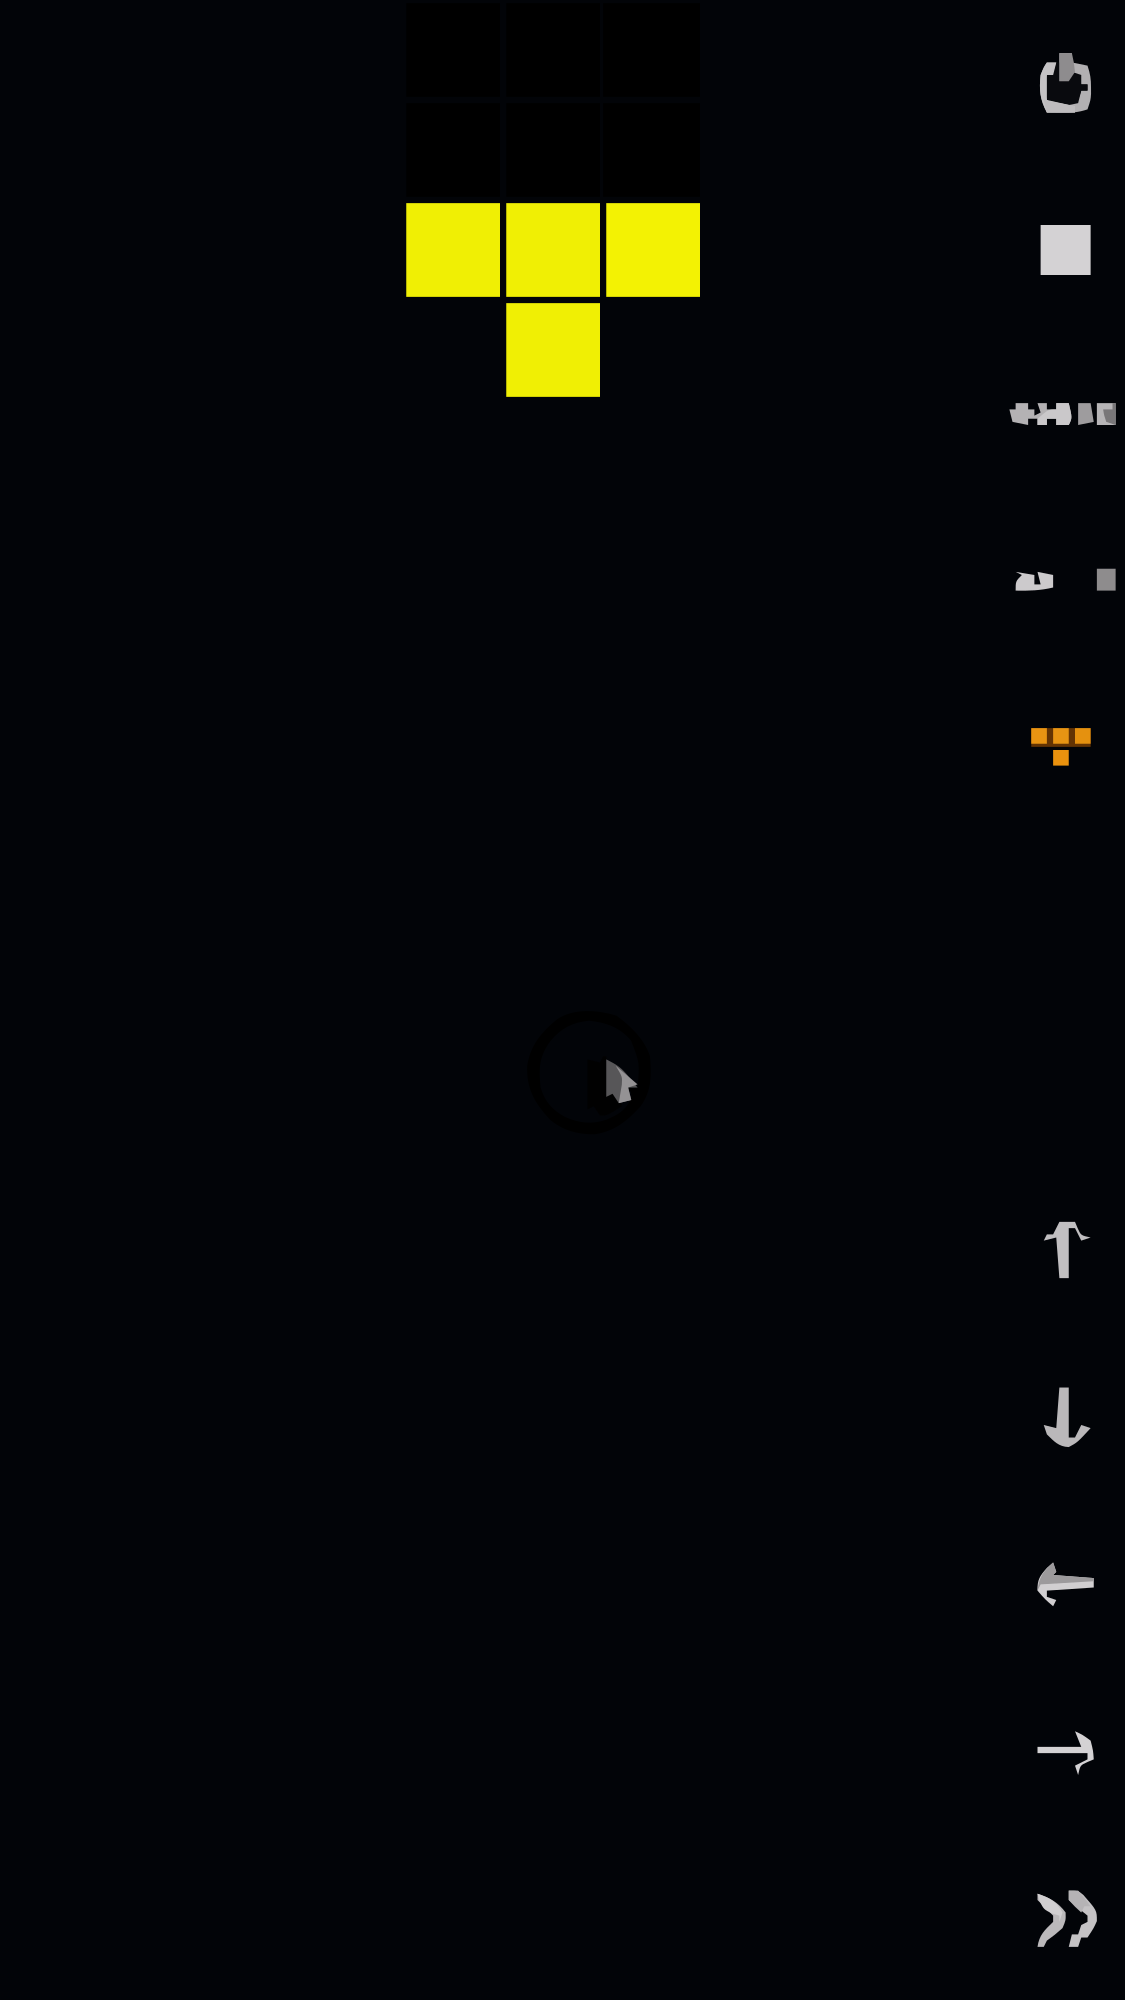
\includegraphics[width=0.3\textwidth]{10-gameCoreGuide-screenshot}
    \\[10pt] % Tạo khoảng cách nhỏ giữa hình và chú thích
    \textit{\small Hình 10.1: Màn hình module gameCore}
\end{figure}
\noindent\textbf{Thay đổi chính trong v2:}

\vspace{4pt}
\begin{tabularx}{\linewidth}{|l|l|X|}
    \hline
    	extbf{Tính năng} & \textbf{V1} & \textbf{V2} \\
    \hline
    Tốc độ rơi       & Cố định 500\,ms & 5 dải theo điểm: 500/400/300/200/100\,ms \\
    \hline
    Soft drop         & Luôn 100\,ms (hằng số) & \texttt{getFallInterval(score) / 5} -- động \\
    \hline
    Điểm xoá dòng    & 1\,pt / dòng & $n^2$ pt ($n$ = số dòng cùng lúc) \\
    \hline
    Hiệu ứng xoá dòng & Tức thì & 3 lần chớp (6 tick $\times$ 80\,ms) trước khi xoá \\
    \hline
    Khối xem trước   & NEXT-1 luôn hiện & NEXT-2/3 mở khoá theo ngưỡng điểm story \\
    \hline
    Màu khối          & 6 màu ngẫu nhiên toàn bộ & Lọc theo \texttt{colorEnabled[7]} từ Console \\
    \hline
    Bàn cờ ban đầu   & Luôn trống & \texttt{tableMatrix} từ story (có thể có ô sẵn) \\
    \hline
    Nhạc nền          & Không có & \texttt{SDL\_AudioStream}, gain = \texttt{cfg.volume} \\
    \hline
    Lưu thành tích   & Không có & \texttt{dbInsertRecord()} + \texttt{dbUpsertStoryProgress()} \\
    \hline
    Sidebar slot 4    & NEXT-1 (hình khối) & NEXT-1 + nhãn \texttt{S\{id\}-C\{id\}} nếu story đang chọn \\
    \hline
\end{tabularx}

\subsection{Bố cục màn hình}
Cửa sổ trò chơi được chia thành hai vùng cố định, đặt cạnh nhau theo chiều ngang:
\begin{itemize}
    \item \textbf{Bảng chơi (Board) -- 240$\times$480 px:} chiếm phần bên trái màn hình. Đây là khu vực các khối Tetromino sẽ rơi xuống. Bảng được chia thành lưới gồm 16 cột $\times$ 32 hàng.
    \item \textbf{Thanh bên (Sidebar) -- 30$\times$480 px:} chiếm phần bên phải màn hình. Thanh bên gồm 12 ô đồng nhất kích thước 30$\times$40 px, hiển thị thông tin trạng thái và các nút điều khiển bằng chuột.
\end{itemize}

\noindent\textbf{Sơ đồ 12 ô của thanh bên} (đánh số từ trên xuống dưới):

\vspace{4pt}
\begin{tabularx}{\linewidth}{|c|l|X|}
    \hline
    \textbf{Ô \#} & \textbf{Tên} & \textbf{Chức năng} \\
    \hline
    0  & QUIT        & Mở hộp thoại thoát game (icon hình nút nguồn). \\
    \hline
    1  & PAUSE       & Tạm dừng hoặc tiếp tục trò chơi. \\
    \hline
    2  & SCORE       & Hiển thị điểm số hiện tại (định dạng 5 chữ số). \\
    \hline
    3  & TIMER       & Hiển thị thời gian chơi tích lũy (định dạng \texttt{HH:MM}). \\
    \hline
    4  & NEXT-1      & Xem trước hình dạng khối tiếp theo sẽ rơi. \\
    \hline
    5  & NEXT-2 & Xem trước khối thứ hai -- \textbf{hiện khi} \texttt{score $\\geq$ cfg.nextBlockScore}
                  (và \texttt{nextBlockScore > 0}). Không hiện nếu chưa chọn story. \\
    \hline
    6  & NEXT-3 & Xem trước khối thứ ba -- \textbf{hiện khi} NEXT-2 đã mở và
                  \texttt{score $\\geq$ nextBlockScore $\\times$ 2} (fallback V2;
                  V3 sẽ dùng ngưỡng riêng từ \texttt{shared\_data}). \\
    \hline
    7  & ARROW UP    & Lật khối theo chiều kim đồng hồ. \\
    \hline
    8  & ARROW DOWN  & Lật khối ngược chiều kim đồng hồ. \\
    \hline
    9  & ARROW LEFT  & Di chuyển khối sang trái. \\
    \hline
    10 & ARROW RIGHT & Di chuyển khối sang phải. \\
    \hline
    11 & SPEED       & Nút tăng tốc rơi (\textit{Speed Booster}). \\
    \hline
\end{tabularx}

\vspace{4pt}
\noindent\textit{Lưu ý:} toàn bộ icon trên thanh bên được vẽ thủ công bằng hình học SDL (\textit{procedural drawing}) thay vì sử dụng ảnh bitmap. Khi bạn nhấn giữ chuột hoặc giữ phím tương ứng, icon sẽ được tô \textbf{vàng nổi bật} (\textit{highlight yellow}) để báo hiệu trạng thái \textit{active}.

\subsection{Quy tắc chơi}
Lối chơi cốt lõi đòi hỏi sự khéo léo và tư duy không gian. Các khối Tetromino sẽ liên tục rơi xuống từ phía trên màn hình, và nhiệm vụ của bạn là sắp xếp chúng để ghi điểm:
\begin{itemize}
    \item \textbf{Lắp ráp các khối} sao cho lấp đầy hoàn toàn một (hoặc nhiều) hàng ngang trên bảng chơi.
    \item \textbf{Xóa hàng (Line Clear):} mỗi khi một hàng ngang được lấp kín, hàng đó sẽ tự động biến mất, các khối phía trên rơi xuống bù chỗ trống. Mỗi hàng được xóa cộng \textbf{1 điểm} vào tổng điểm.
    \item \textbf{Game Over:} nếu khối mới sinh ra không còn chỗ trống ở đỉnh bảng (chạm khối đã có trên bảng), trò chơi sẽ kết thúc và tự động mở \textit{hộp thoại Game Over}.
\end{itemize}

\noindent\textbf{Bộ khối hình:} Phiên bản v1 sử dụng 5 khối cơ bản: \textbf{L}, \textbf{I}, \textbf{Z}, \textbf{O}, \textbf{T}. Để tăng tính đa dạng, mỗi khối khi sinh ra sẽ có \textbf{50\% xác suất bị lật gương theo trục X} (\textit{mirror flip}); nhờ đó bạn có thể bắt gặp các biến thể trông giống J (lật L) hoặc S (lật Z) mà không cần khai báo riêng.

\noindent\textbf{Bộ màu sắc:} Mỗi khối được tô ngẫu nhiên một trong 6 màu: \textit{Xanh dương, Đỏ, Xanh lá, Vàng, Cam, Tím}.

\noindent\textbf{Thay đổi v2 -- bảng màu cấu hình được:}
Từ v2, màu khối \textbf{không luôn luôn là 6 màu cố định}. Mảng
\texttt{colorEnabled[7]} (được thiết lập ở popup Settings của gameConsole)
kiểm soát màu nào được phép xuất hiện:

\vspace{4pt}
\begin{tabularx}{\linewidth}{|c|l|l|}
    \hline
    \textbf{Index} & \textbf{Màu} & \textbf{Ánh xạ sang \texttt{COLORS[]}} \\
    \hline
    0 & Đỏ    & \texttt{COLORS[2]} \\
    \hline
    1 & Cam   & \texttt{COLORS[5]} \\
    \hline
    2 & Hồng  & \texttt{COLORS[7]} \\
    \hline
    3 & Vàng  & \texttt{COLORS[4]} \\
    \hline
    4 & Xanh lá & \texttt{COLORS[3]} \\
    \hline
    5 & Xanh dương & \texttt{COLORS[1]} \\
    \hline
    6 & Tím   & \texttt{COLORS[6]} \\
    \hline
\end{tabularx}

\vspace{4pt}
\noindent Nếu tất cả index bị tắt (không thể xảy ra do Console guard "at least 1"),
hệ thống fallback về toàn bộ 6 màu gốc -- gameCore không bao giờ crash do
\texttt{enabledIndices} rỗng.

\subsection{Hệ thống điều khiển}

\subsubsection{Điều khiển bằng bàn phím}
Bàn phím là kênh điều khiển chủ đạo trên môi trường desktop. Hệ thống chấp nhận song song hai cụm phím (mũi tên và WASD) để bạn dùng tay nào cũng được:

\vspace{4pt}
\begin{tabularx}{\linewidth}{|l|X|}
    \hline
    \textbf{Phím} & \textbf{Hành động} \\
    \hline
    \texttt{A} \,/\, \texttt{$\leftarrow$}     & Di chuyển khối sang \textbf{trái}. \\
    \hline
    \texttt{D} \,/\, \texttt{$\rightarrow$}    & Di chuyển khối sang \textbf{phải}. \\
    \hline
    \texttt{W} \,/\, \texttt{$\uparrow$}       & Lật khối \textbf{theo chiều kim đồng hồ}. \\
    \hline
    \texttt{S} \,/\, \texttt{$\downarrow$}     & Lật khối \textbf{ngược chiều kim đồng hồ}. \\
    \hline
    \texttt{SPACE}                              & Bật chế độ \textbf{rơi nhanh} (Soft Drop) khi giữ phím. \\
    \hline
    \texttt{ENTER} \,/\, \texttt{KP\_ENTER}     & Tạm dừng hoặc tiếp tục trò chơi. \\
    \hline
    \texttt{ESC}                                & Mở hộp thoại Quit. \\
    \hline
\end{tabularx}

\vspace{4pt}
\noindent\textit{Lưu ý quan trọng:} nếu thao tác di chuyển hoặc xoay khiến khối va vào tường, đáy bảng hoặc một khối đã đặt cố định, hệ thống sẽ \textbf{tự động hủy thao tác} đó để tránh đè khối. Bạn có thể yên tâm spam phím xoay sát tường mà không lo phá bố cục bàn cờ.

\subsubsection{Điều khiển bằng chuột}
Toàn bộ chức năng có thể thực hiện chỉ với chuột, hữu ích khi bạn chơi trên laptop không có numpad hoặc khi đang tay cầm cốc cà phê. Cơ chế \textbf{Click \& Hold} (nhấn và giữ) được hỗ trợ cho các nút điều hướng và nút Speed Booster:
\begin{itemize}
    \item \textbf{Click vào icon QUIT} (ô số 0): mở hộp thoại Quit, tương đương phím \texttt{ESC}.
    \item \textbf{Click vào icon PAUSE} (ô số 1): tạm dừng hoặc tiếp tục, tương đương phím \texttt{ENTER}.
    \item \textbf{Click các nút mũi tên} (ô 7--10): mỗi cú click thực hiện một thao tác (lật/di chuyển), tương đương nhấn phím mũi tên một lần.
    \item \textbf{Giữ chuột nút Speed Booster} (ô 11): bật chế độ rơi nhanh suốt thời gian giữ, tương đương giữ phím \texttt{SPACE}.
\end{itemize}

Khi nút đang được giữ, icon sẽ chuyển sang \textbf{màu vàng nổi bật} để bạn biết hệ thống đã ghi nhận thao tác.

\subsubsection{Điều khiển bằng cử chỉ vuốt (cảm ứng)}
Trên thiết bị cảm ứng (điện thoại, máy tính bảng, hoặc trình duyệt hỗ trợ touch), bạn có thể thao tác trực tiếp ngay trên \textit{vùng bảng chơi} mà không cần chạm vào thanh bên:

\vspace{4pt}
\begin{tabularx}{\linewidth}{|l|X|}
    \hline
    \textbf{Cử chỉ} & \textbf{Hành động} \\
    \hline
    Vuốt \textbf{ngang} (trái/phải) trên \textit{khối đang rơi} & Di chuyển khối sang trái/phải. \\
    \hline
    Vuốt \textbf{dọc} (lên/xuống) trên \textit{nền bảng} (không trúng khối) & Lật khối ngược/theo chiều kim đồng hồ. \\
    \hline
\end{tabularx}

\vspace{4pt}
\noindent\textbf{Quy tắc nhận diện:}
\begin{itemize}
    \item Cử chỉ chỉ được ghi nhận khi quãng vuốt đạt tối thiểu \textbf{15 px}, để tránh nhầm lẫn với thao tác chạm (\textit{tap}).
    \item Hệ thống xét \textit{trục ưu thế}: nếu khoảng vuốt ngang lớn hơn dọc thì coi là vuốt ngang, và ngược lại; vuốt chéo gần 45° sẽ bị bỏ qua.
    \item Vuốt trên \textbf{thanh bên} (vùng \texttt{x $\geq$ 240}) không kích hoạt cử chỉ -- thanh bên giữ nguyên hành vi tap như bình thường.
\end{itemize}

\subsection{Các tính năng nâng cao}

\subsubsection{Rơi nhanh (Soft Drop)}
Khi muốn nhanh chóng kết thúc một hàng hoặc đặt khối vào vị trí đã chọn sẵn, bạn có thể bật chế độ rơi nhanh:
\begin{itemize}
    \item \textbf{Trên bàn phím:} nhấn giữ phím \texttt{SPACE}.
    \item \textbf{Trên chuột/cảm ứng:} nhấn giữ nút \textit{Speed Booster} (ô số 11).
\end{itemize}
Trong thời gian giữ, tốc độ rơi của khối tăng lên \textbf{5 lần} so với bình thường (chu kỳ rơi giảm từ 500 ms xuống 100 ms). Khi nhả phím/chuột, tốc độ trở về mặc định ngay lập tức.

\subsubsection{Đồng hồ tính giờ chơi (Play Timer)}
Ô số 3 trên thanh bên hiển thị tổng thời gian chơi \textbf{thực tế} theo định dạng \texttt{HH:MM} (giờ:phút). Đồng hồ chỉ đếm khi trò chơi đang chạy: nếu bạn tạm dừng hoặc mở hộp thoại Quit, đồng hồ sẽ \textbf{ngừng đếm}, và tiếp tục từ giá trị cũ khi quay lại. Nhờ đó, thời gian hiển thị phản ánh đúng nỗ lực thực tế, không bị ``ăn gian'' vì pause lâu.

\subsubsection{Hệ thống điểm số}
\begin{itemize}
    \item \textbf{Quy tắc tính điểm:} mỗi hàng được xóa = \textbf{1 điểm}.
    \item \textbf{Điểm tối đa:} \texttt{99999} (5 chữ số). Vượt mức này, điểm sẽ được giữ nguyên ở \texttt{99999}.
    \item \textbf{Định dạng hiển thị:} luôn là chuỗi 5 chữ số có đệm số 0 ở trước (ví dụ: \texttt{00007}, \texttt{00125}, \texttt{99999}). Định dạng cố định này giúp ô SCORE và ô TIMER có cùng kích thước hiển thị, cân đối hài hòa trong không gian hẹp 30$\times$40 px.
\end{itemize}

\subsubsection{Xem trước khối tiếp theo (Preview Next)}
Ô \textbf{NEXT-1} (ô số 4) hiển thị thu nhỏ hình dạng của khối sắp rơi tiếp theo, kèm đúng màu sẽ được sinh ra. Nhờ đó, bạn có thể \textbf{lập kế hoạch trước một bước}, sắp xếp khối hiện tại ở vị trí tối ưu để đón khối kế tiếp.

\subsubsection{Tạm dừng / Tiếp tục (Pause / Play)}
Bạn có thể tạm dừng trò chơi bất cứ lúc nào theo một trong ba cách: nhấn phím \texttt{ENTER}, phím \texttt{KP\_ENTER} trên numpad, hoặc click vào icon PAUSE (ô số 1). Khi trạng thái thay đổi, icon trên thanh bên cũng đổi tương ứng để bạn dễ nhận biết:
\begin{itemize}
    \item \textbf{Hình vuông đặc} -- trò chơi \textit{đang chạy} (click để dừng).
    \item \textbf{Hình tam giác} -- trò chơi \textit{đang tạm dừng} (click để tiếp tục).
\end{itemize}
Trong thời gian tạm dừng, đồng hồ play timer ngừng đếm và khối ngừng rơi.

\subsection{Độ khó tăng dần theo điểm số -- v2}
Thay thế hằng số \texttt{FALL\_INTERVAL\_NORMAL = 500} của v1, tốc độ rơi
được tính \textbf{động mỗi frame} bởi hàm \texttt{getFallInterval(score)}:

\vspace{4pt}
\begin{tabularx}{\linewidth}{|c|c|c|c|}
    \hline
    \textbf{Dải điểm} & \textbf{Fall interval} & \textbf{Soft drop} & \textbf{Cảm nhận} \\
    \hline
    0 -- 4   & 500\,ms & 100\,ms & Tốc độ học, khởi động \\
    \hline
    5 -- 14  & 400\,ms &  80\,ms & Nhịp chơi bình thường \\
    \hline
    15 -- 29 & 300\,ms &  60\,ms & Bắt đầu căng thẳng \\
    \hline
    30 -- 49 & 200\,ms &  40\,ms & Tốc độ cao, phản xạ \\
    \hline
    50+      & 100\,ms &  20\,ms & Giới hạn khả năng người \\
    \hline
\end{tabularx}

\vspace{4pt}
\noindent\textit{Lưu ý kỹ thuật:} tỉ lệ \textbf{soft drop = 1/5 fall interval} được giữ
nguyên xuyên suốt mọi dải điểm (không còn hằng số cứng \texttt{FALL\_INTERVAL\_FAST}).
Khi khối đang trong pha flash (\texttt{pendingClear = true}), bộ đếm
\texttt{lastFallTime} bị đóng băng -- khối không rơi trong 6 tick $\times$ 80\,ms
$\approx$ 480\,ms của hiệu ứng chớp. Đây là hành vi chủ ý: người chơi có
thời gian quan sát trước khi dòng biến mất.

\subsection{Hiệu ứng xoá dòng và điểm thưởng -- v2}

\subsubsection{Hiệu ứng chớp tắt (Flash Effect)}
Thay vì xoá hàng tức thì như v1, v2 thêm giai đoạn phản hồi thị giác
trước khi hàng thực sự biến mất:

\begin{enumerate}
    \item \texttt{lockBlock()} phát hiện hàng đầy → lưu vào \texttt{clearRows[]},
        bật \texttt{pendingClear = true}.
    \item Vòng lặp chính chớp hàng đó \textbf{luân phiên trắng/tối} mỗi 80\,ms.
    \item Sau đúng 6 tick (3 lần trắng + 3 lần tối $\approx$ 480\,ms),
        \texttt{finishLineClear()} thực hiện xoá thật và cộng điểm.
    \item Fall timer được reset ngay sau khi xoá -- không bị ăn thời gian chờ.
\end{enumerate}

\subsubsection{Điểm thưởng xoá nhiều dòng cùng lúc}
V2 áp dụng hệ số $n^2$ thay vì cộng tuyến tính:

\vspace{4pt}
\begin{tabularx}{\linewidth}{|c|c|c|X|}
    \hline
    \textbf{Số dòng ($n$)} & \textbf{V1} & \textbf{V2} & \textbf{Chiến thuật} \\
    \hline
    1 & 1\,pt & 1\,pt  & Không đổi \\
    \hline
    2 & 2\,pt & 4\,pt  & Lợi $2\\times$ so với xoá lẻ \\
    \hline
    3 & 3\,pt & 9\,pt  & Lợi $3\\times$ \\
    \hline
    4 & 4\,pt & 16\,pt & Lợi $4\\times$ -- \textit{Tetris bonus} \\
    \hline
\end{tabularx}

\vspace{4pt}
\noindent Giới hạn điểm vẫn là \texttt{99999} (5 chữ số). Việc tích lũy 4 dòng cùng lúc
tăng tốc độ rơi nhanh hơn, tạo vòng lặp tự nhiên: \textit{thưởng lớn} $\Rightarrow$
\textit{khó hơn ngay} -- khuyến khích chiến thuật giữ hàng đợi Tetris.

\subsection{Xem trước 3 khối và điều kiện mở khoá -- v2}
V1 chỉ hiện \textbf{NEXT-1} cố định. V2 bổ sung hàng đợi 3 khối
(\texttt{nextBlock}, \texttt{nextBlock2}, \texttt{nextBlock3}) và
cơ chế mở khoá ô 5/6 theo tiến trình tuyến truyện:

\vspace{4pt}
\begin{tabularx}{\linewidth}{|l|l|X|}
    \hline
    \textbf{Slot} & \textbf{Điều kiện hiển thị} & \textbf{Ghi chú} \\
    \hline
    \textbf{NEXT-1} (ô 4) & Luôn hiện & Hành vi v1 giữ nguyên. \\
    \hline
    \textbf{NEXT-2} (ô 5) & \texttt{cfg.nextBlockScore > 0}
                     \textbf{và} \texttt{score $\\geq$ nextBlockScore}
                   & \texttt{nextBlockScore} đọc từ \texttt{shared\_data}
                     qua \texttt{SettingsConfig} khi chọn story. \\
    \hline
    \textbf{NEXT-3} (ô 6) & NEXT-2 đã mở
                     \textbf{và} \texttt{score $\\geq$ nextBlockScore $\\times$ 2}
                   & Ngưỡng $\\times$2 là fallback V2; V3 sẽ thêm
                     trường riêng trong \texttt{shared\_data}. \\
    \hline
\end{tabularx}

\vspace{4pt}
\noindent Khi \texttt{cfg.nextBlockScore == 0} (không chọn story), chỉ NEXT-1 hiện --
hành vi v1 được bảo toàn hoàn toàn. Mỗi lần khóa khối
(\texttt{lockBlock()} $\\rightarrow$ \texttt{finishLineClear()}),
hàng đợi dịch chuyển: NEXT-2 $\\rightarrow$ vị trí NEXT-1,
NEXT-3 $\\rightarrow$ NEXT-2, và \texttt{spawnBlock()} sinh một khối mới vào NEXT-3.

\subsection{Bàn cờ khởi tạo từ tuyến truyện (tableMatrix) -- v2}
Mỗi story trong \texttt{shared\_data} có thể định nghĩa trạng thái bàn cờ
ban đầu thông qua trường \texttt{tableMatrix}. Khi \texttt{resetGame()} được gọi
(lần đầu vào gameCore hoặc Restart), hệ thống đọc \texttt{cfg.tableMatrix} và
điền sẵn các ô màu \textbf{trước khi} sinh khối đầu tiên.

\noindent\textbf{Định dạng chuẩn (V2):}
Các hàng ngăn cách bởi dấu chấm phẩy (\texttt{;}), các cột ngăn cách bởi
dấu phẩy (\texttt{,}), giá trị = colorID (0 = trống, 1--7 = màu tương ứng):
\begin{verbatim}
"0,0,1,2,0,0,3,0,0,1;0,2,2,1,3,1,2,0,1,2"
\end{verbatim}
Chuỗi trên tạo 2 hàng đáy được điền sẵn.
Chuỗi rỗng (\texttt{""}) = bàn trống như v1.

\noindent\textbf{Căn lề:} các hàng trong \texttt{tableMatrix} được đặt \textit{sát đáy}
(\texttt{BOARD\_ROWS - rowCount}). Parse lỗi (giá trị ngoài 0--7,
sai số cột) bị bỏ qua từng ô, không crash.

\subsection{Nhạc nền -- v2}
Khi vào \texttt{runGameCore()}, hệ thống mở một \texttt{SDL\_AudioStream} silent
(\texttt{coreOpenBgm(cfg.volume)}) và áp dụng gain ngay lập tức:
\begin{itemize}
    \item \textbf{Gain = cfg.volume}: âm lượng kế thừa trực tiếp từ slider
        trong popup Settings của gameConsole -- không cần người chơi cài lại.
    \item \textbf{Phạm vi}: \texttt{[0.0 .. 1.0]}, áp dụng qua
        \texttt{SDL\_SetAudioStreamGain()} (SDL3 native, không dùng SDL\_mixer).
    \item \textbf{Cleanup}: \texttt{coreCloseBgm()} được gọi khi
        \texttt{runGameCore()} trả về -- không rò stream giữa các lần
        Console $\\leftrightarrow$ Core round-trip.
    \item \textbf{Headless/no-audio}: nếu không có thiết bị âm thanh,
        \texttt{g\_coreBgmStream} là \texttt{nullptr} và gain call là no-op --
        không crash trên môi trường CI hoặc Docker.
\end{itemize}
\noindent V2 chưa nạp file nhạc thực sự (stub silent). Kiến trúc sẵn sàng: khi
có file nhạc, chỉ cần queue sample vào stream hiện tại mà không cần thay đổi
volume logic hay signature.

\subsection{Trạng thái đặc biệt}

\subsubsection{Hộp thoại Quit / Game Over (Lightbox)}
Hộp thoại này được hiển thị theo kỹ thuật \textit{lightbox}: nền phía sau bị phủ mờ đen để tập trung sự chú ý vào popup ở giữa. Hộp thoại tự động kích hoạt trong các trường hợp:
\begin{itemize}
    \item Bạn nhấn phím \texttt{ESC} hoặc click icon QUIT.
    \item Trò chơi kết thúc do khối mới không có chỗ sinh ra (\textit{Game Over}).
\end{itemize}

\noindent\textbf{Thông tin hiển thị trong hộp thoại:}
\begin{itemize}
    \item Tiêu đề trạng thái: \texttt{PAUSED} (khi do người chơi mở) hoặc \texttt{GAME OVER} (khi do thua).
    \item \textbf{Current score} -- điểm số hiện tại.
    \item \textbf{Total time} -- tổng thời gian chơi thực tế (loại trừ pause), định dạng \texttt{HH:MM:SS}.
\end{itemize}

\noindent\textbf{Bốn lựa chọn hành động:}
\begin{itemize}
    \item \textbf{Restart} -- bắt đầu một ván mới ngay trong gameCore (reset điểm và đồng hồ).
    \item \textbf{Console} -- thoát gameCore và quay lại màn hình \textit{gameConsole} (menu chính).
    \item \textbf{Quit} -- thoát hoàn toàn ứng dụng (trên web sẽ chuyển sang màn hình Reload, xem mục tiếp).
    \item \textbf{Cancel} -- đóng hộp thoại và quay lại trận đấu (nếu chưa Game Over).
\end{itemize}
Ngoài ra, bạn có thể click vào nút \textbf{X} màu đỏ ở góc trên bên phải hộp thoại để đóng nhanh -- tương đương Cancel.

\noindent\textbf{Thay đổi v2 -- tự động lưu thành tích:}
Từ v2, \textbf{mọi con đường thoát khỏi một phiên chơi} đều kích hoạt ghi DB
trước khi thực hiện hành động:

\vspace{4pt}
\begin{tabularx}{\linewidth}{|l|X|}
    \hline
    \textbf{Hành động} & \textbf{Chuỗi thực hiện} \\
    \hline
    \textbf{Game Over} (tự động) & Vòng lặp chính phát hiện
        \texttt{isGameOver \&\& !gameOverRecorded} $\\rightarrow$
        gọi \texttt{onGameOver()} $\\rightarrow$ set flag. \\
    \hline
    \textbf{Restart} & Kiểm tra flag trước khi \texttt{resetGame()} --
        ghi record kể cả khi score = 0 (phiên chơi hợp lệ). \\
    \hline
    \textbf{Console / Quit} & Kiểm tra flag trước khi trả về --
        đảm bảo không mất dữ liệu khi thoát sớm. \\
    \hline
\end{tabularx}

\vspace{4pt}
\noindent Flag \texttt{gameOverRecorded} (kiểu \texttt{bool}, local trong
\texttt{runGameCore()}) đóng vai trò \textit{idempotency guard}: dù ba đường
thoát có thể hội tụ về cùng \texttt{onGameOver()}, hàm chỉ chạy \textbf{đúng
một lần} mỗi phiên. WASM: \texttt{FS.syncfs(false)} được gọi sau mỗi write
để flush xuống IndexedDB.

\subsubsection{Màn hình Reload (chỉ trên Web/WASM)}
Trên trình duyệt, lệnh \texttt{exit()} của ứng dụng C++ không thể đóng tab thực sự. Để thay thế, sau khi bạn chọn \textbf{Quit} từ hộp thoại, gameCore hiển thị một \textbf{màn hình đen} với một nút \textbf{RELOAD} lớn ở giữa kèm dòng chú thích \textit{``Press F5 or click RELOAD to start a new game''}.

Bạn có thể kích hoạt làm mới trang theo bốn cách:
\begin{itemize}
    \item Click chuột vào nút RELOAD.
    \item Nhấn phím \texttt{F5}.
    \item Nhấn \texttt{ENTER} hoặc \texttt{SPACE}.
\end{itemize}
Khi đó, trình duyệt sẽ tải lại trang và bạn được khởi động lại từ màn hình gameStory đầu tiên. Trên phiên bản desktop, \textbf{Quit} sẽ đóng cửa sổ ngay lập tức và không hiển thị màn hình này.

\subsection{Lưu thành tích vào cơ sở dữ liệu -- v2}
Hàm \texttt{onGameOver()} thực hiện 3 bước theo thứ tự:

\begin{enumerate}
    \item \textbf{dbOpen("default")} -- mở file \texttt{default.sqlite}
        tại \texttt{SDL\_GetPrefPath("uit","cTetris")}. gameCore \textit{không
        sở hữu} DB connection lâu dài -- mở, dùng, đóng trong cùng một lần gọi.
    \item \textbf{dbInsertRecord(rec)} -- ghi một hàng vào
        \texttt{default\_Records} với các trường:
\end{enumerate}

\vspace{4pt}
\begin{tabularx}{\linewidth}{|l|l|X|}
    \hline
    \textbf{Trường} & \textbf{Nguồn} & \textbf{Mô tả} \\
    \hline
    \texttt{idUser}       & \texttt{"default"} & ID người dùng V2 cố định. \\
    \hline
    \texttt{startTS}      & \texttt{state.gameStartTime} & Mốc bắt đầu (Uint32 ms). \\
    \hline
    \texttt{endTS}        & \texttt{SDL\_GetTicks()} & Mốc kết thúc. \\
    \hline
    \texttt{idStory/Chapter} & \texttt{s\_cfg} & Story đang chơi (0 nếu không chọn). \\
    \hline
    \texttt{totalScore}   & \texttt{state.score} & Điểm tại thời điểm kết thúc. \\
    \hline
    \texttt{totalSeconds} & \texttt{elapsedMs/1000} & Thời gian chơi thực tế. \\
    \hline
    \texttt{avgSpeed}     & \texttt{score/totalSeconds} & Tốc độ trung bình. \\
    \hline
    \texttt{retryNo}      & \texttt{state.retryCount} & Số lần Restart trong phiên. \\
    \hline
\end{tabularx}

\begin{enumerate}\setcounter{enumi}{2}
    \item \textbf{dbUpsertStoryProgress()} + \textbf{dbCheckAndUnlockStories()} --
        nếu \texttt{storyId > 0}, cập nhật \texttt{lastMaxScore}/\texttt{lastMaxSpeed}/
        \texttt{totalRetries} và cascade-unlock các story kế tiếp đủ điều kiện.
        Lần mở Stories popup tiếp theo trong Console sẽ phản chiếu kết quả này
        từ DB -- không có cache stale.
\end{enumerate}

\noindent\textit{Lưu ý V3:} tính năng đồng bộ thành tích lên \textbf{Cloudflare D1}
(\texttt{d1\_board}) qua Cloudflare Worker sẽ được thêm ở V3 (Task 3.2).
Bảng \texttt{sync\_Records} trong SQLite local đóng vai trò staging area --
Board popup trong gameConsole hiển thị dữ liệu từ đây.

\subsection{Giới hạn còn lại sau v2}
\begin{itemize}
    \item \textbf{Nhạc nền thực sự}: stream đã mở và gain đã hoạt động,
        nhưng chưa có file nhạc được queue -- v3 sẽ bổ sung.
    \item \textbf{Đồng bộ thành tích lên Cloudflare D1}: hiện lưu local
        SQLite; V3 Task 3.2 sẽ POST lên \texttt{d1\_board} qua
        Cloudflare Worker sau mỗi game over.
    \item \textbf{NEXT-3 ngưỡng riêng}: V2 dùng \texttt{nextBlockScore $\\times$ 2}
        làm fallback; V3 sẽ thêm trường \texttt{nextBlockScore3} vào
        \texttt{shared\_data} và \texttt{SettingsConfig}.
    \item \textbf{Nhập tên người chơi}: V3 Task 3.1 sẽ thêm text input vào
        popup Game Over để ghi \texttt{nameUser} vào record trước khi submit.
    \item \textbf{Sidebar ô NEXT-1}: nhãn \texttt{S\{id\}-C\{id\}} hiện render
        đè lên góc trên của ô NEXT-1 -- V3 sẽ tách thành ô info riêng khi
        layout sidebar được cơ cấu lại.
\end{itemize}

\label{LastPageGameCoreGuide}
\end{document}